\section{More data points}
\label{apx_more_data_points}

This dissertation evaluated \gls{upnp} and \gls{mqttd} deployments under different configurations of \textit{devices} and \textit{control-points}. The number of entities was increased incrementally from 1 to 10 in unit steps, and from 10 to 100 in steps of ten. For the sake of readability, Section \ref{sec_experimental_results} reports only the graphs corresponding to the data points 1, 5, 10, 50, and 100. This appendix presents the complete set of collected data.

\subsection{\gls{upnp}}
%\subsubsection{\gls{upnp} latency}
\begin{figure}[!ht]
    \centering
    \subfloat[]{
\includegraphics[width=0.48\linewidth]{results/upnp_latency.png}
    \label{fig_apx_upnp_latency_wireless}}
    \hfil
    \subfloat[]{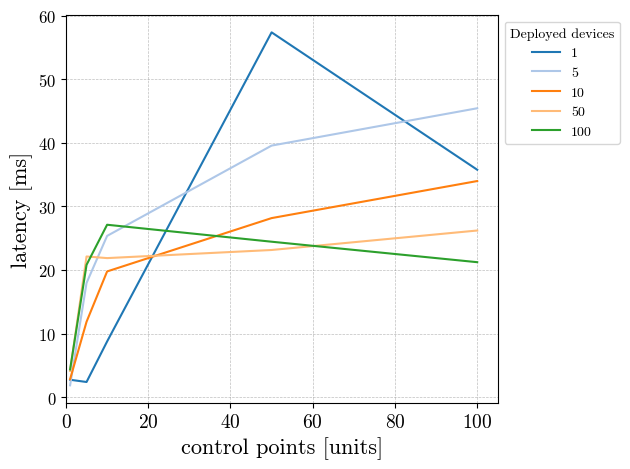
\includegraphics[width=0.48\linewidth]{results/wired_upnp_latency.png}
    \label{fig_apx_upnp_latency_cabled}}
    \caption{\gls{upnp} (a) wireless and (b) wired latency}
    \label{fig_apx_upnp_latency}
\end{figure}

%\begin{figure}[!ht]
%    \centering
%    \subfloat[]{
\includegraphics[width=0.48\linewidth]{results/upnp_0_latency_light.png}
%    \label{fig_apx_upnp_0_latency}}
%    \hfil
%    \subfloat[]{
\includegraphics[width=0.48\linewidth]{results/upnp_0_robustness_light.png}
%    \label{fig_apx_upnp_0_robustness}}
%    \caption{\gls{upnp} (a) latency and (b) robustness with no random delay}
%    \label{fig_apx_upnp_0}
%\end{figure}

%\subsubsection{\gls{upnp} robustness}
\begin{figure}[!ht]
    \centering
    \subfloat[]{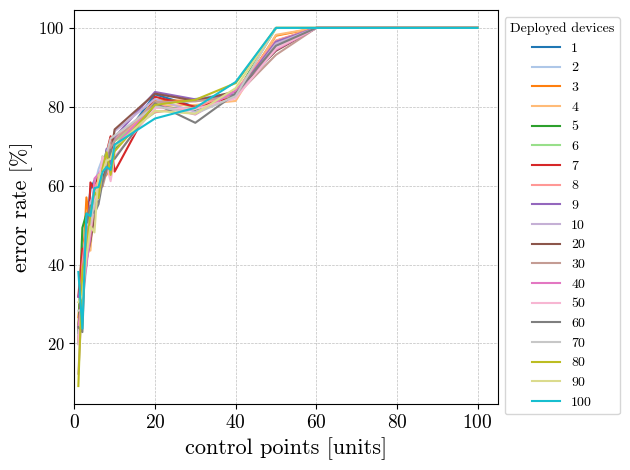
\includegraphics[width=0.48\linewidth]{results/upnp_robustness.png}
    \label{fig_apx_upnp_robustness_wireless}}
    \hfil
    \subfloat[]{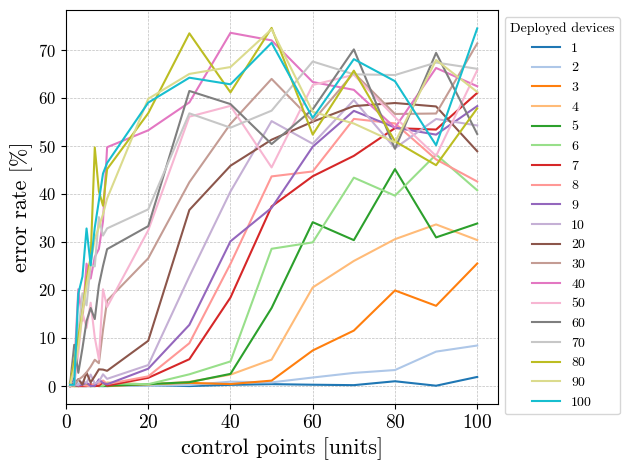
\includegraphics[width=0.48\linewidth]{results/wired_upnp_robustness.png}
    \label{fig_apx_upnp_robustness_cabled}}
    \caption{\gls{upnp} (a) wireless and (b) wired robustness}
    \label{fig_apx_upnp_robustness}
\end{figure}


\subsection{\gls{mqtt}}
%\subsubsection{Latency}
%\begin{figure}[!ht]
%    \centering
%    \subfloat[]{
\includegraphics[width=1\linewidth]{results/mqtt_latency.png}
%    \label{fig_apx_mqtt_latency_wireless}}
%    \\
%    \subfloat[]{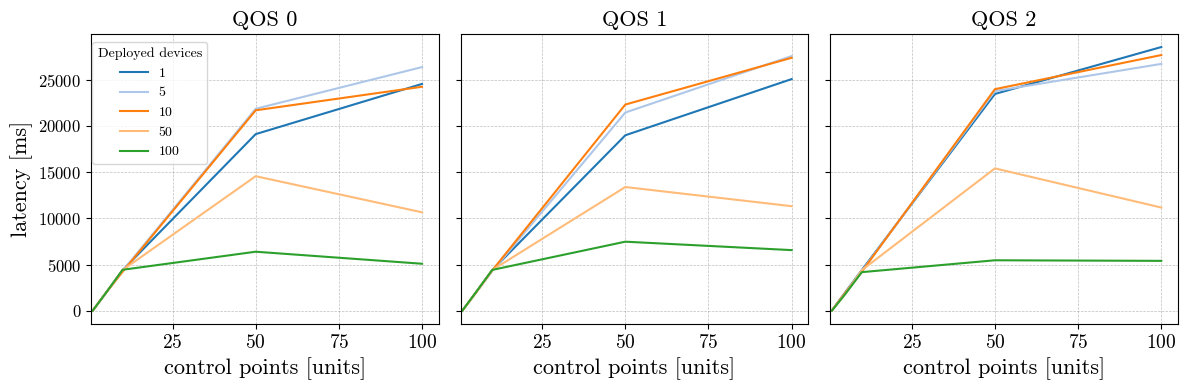
\includegraphics[width=1\linewidth]{results/wired_mqtt_latency_light.png}}
%    \label{fig_apx_mqtt_latency_wired}
%   \caption{\gls{mqtt} latency}
%    \label{fig_apx_mqtt_latency}
%\end{figure}

\begin{figure}[!ht]
    \centering
    
\includegraphics[width=1\linewidth]{results/mqtt_latency.png}
    \caption{\gls{mqtt} latency}
    \label{fig_apx_mqtt_latency_wireless}
\end{figure}

%\subsubsection{Robustness}
%\begin{figure}[!ht]
%    \centering
%    \subfloat[]{
\includegraphics[width=1\linewidth]{results/mqtt_robustness.png}
%    \label{fig_apx_mqtt_robustness_wireless}}
%    \\
%    \subfloat[]{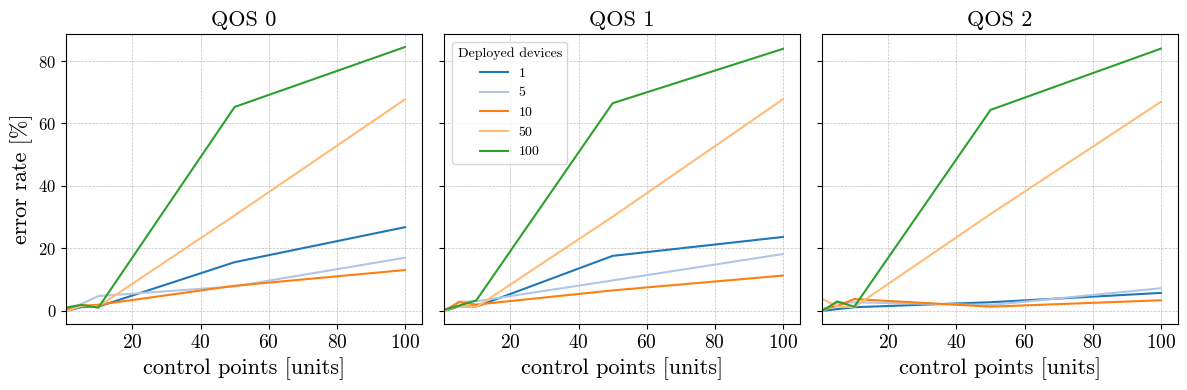
\includegraphics[width=1\linewidth]{results/wired_mqtt_robustness_light.png}
%    \label{fig_apx_mqtt_robustness_wired}}
%    \caption{\gls{mqtt} robustness}
%    \label{fig_apx_mqtt_robustness}
%\end{figure}

\begin{figure}[!ht]
    \centering
    
\includegraphics[width=1\linewidth]{results/mqtt_robustness.png}
    \caption{\gls{mqtt} robustness}
    \label{fig_apx_mqtt_robustness_wireless}
\end{figure}